\section{\K 信号运算}
\subsection{\K 比例运算}

\begin{wrapfigure}{r}{0.25\textwidth}
    \centering
    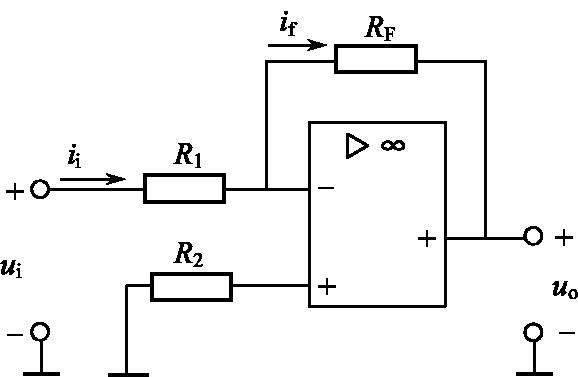
\includegraphics[width=0.25\textwidth]{反相比例运算电路.jpg}
    \caption{反相比例运算电路}
    \label{fig:反相比例运算电路}
\end{wrapfigure}
\Par 对于如图\ref{fig:反相比例运算电路}所示的比例运算电路,我们知道它工作在放大区,关于它是如何实现比例远算的,分析如下:首先我们知道工作在放大区,它就满足虚断现象,因此
\begin{equation*}
    i_+=i_-=0
\end{equation*}
由于$R_2$接地,因此$V_+=0$,而根据虚短原则
\begin{equation*}
    u_+=u_-=0
\end{equation*}
因此输入的电流$i_i$全部流向了$i_f$,它就满足
\begin{equation}
    i_i=\frac{u_i-u_-}{R_1}=i_f=\frac{u_--u_o}{R_F}\xRightarrow{u_-=0}u_o=-\frac{R_F}{R_1}u_i
\end{equation}
可见,它实现了反相比例运算,比例由$R_F/R_1$决定.同时需要指出
\begin{equation}
    R_2=R_1\pll R_F=\frac{1}{\frac{1}{R_1}+\frac{1}{R_F}}
\end{equation}
记下即可.

\begin{wrapfigure}{r}{0.25\textwidth}
    \centering
    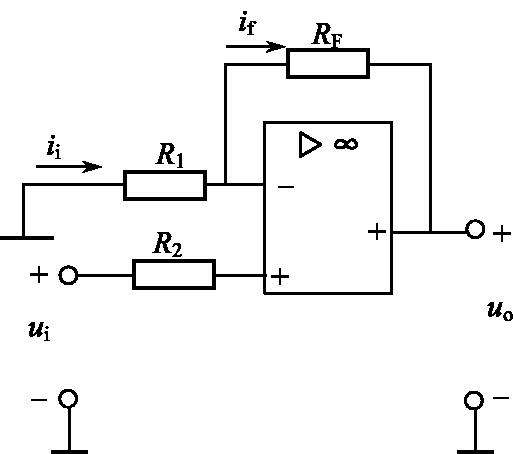
\includegraphics[width=0.25\textwidth]{同相比例运算电路.jpg}
    \caption{同相比例运算电路}
    \label{fig:同相比例运算电路}
\end{wrapfigure}
\Par 既然有反向比例运算电路,那就有同相比例运算电路,电路图如图\ref{fig:同相比例运算电路}所示,这里我们直接放出结果
\begin{equation}
    A_{uf}=\frac{u_o}{u_i}=1+\frac{R_F}{R_1}
\end{equation}
可见,同相比例运算电路的最小放大倍数就是一倍.当$R_1\rightarrow \infty ,R_F\rightarrow 0,R_2\rightarrow 0$时,可以知道$u_o=u_i$,此时它被称为\textbf{电压跟随器},它可以将输入电压与输出电压耦合,防止两者相互影响.

\subsection{\K 加法运算}

\begin{wrapfigure}[9]{r}{0.25\textwidth}
    \centering
    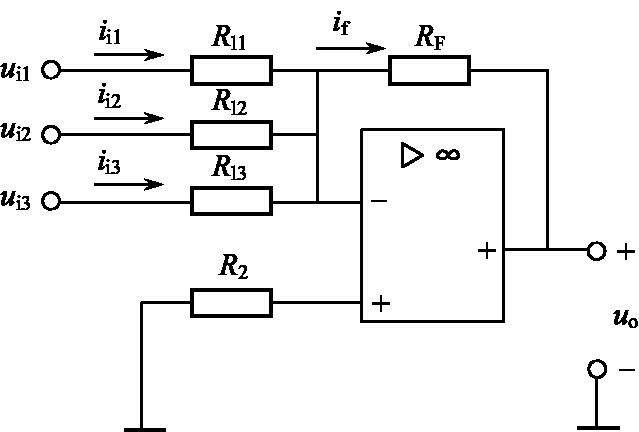
\includegraphics[width=0.25\textwidth]{加法运算电路.jpg}
    \caption{加法运算电路}
    \label{fig:加法运算电路}
\end{wrapfigure}
\Par 加法运算电路如图\ref{fig:加法运算电路}所示,这里我们同样直接给出结果
\begin{equation}
    u_o=-R_F\left( \frac{u_{i1}}{R_{11}}+\frac{u_{i2}}{R_{12}}+\frac{u_{i3}}{R_{13}} \right) 
\end{equation}
此时我们仅需让$R_F=R_{11}=R_{12}=R_{13}$即可实现反相加法运算.
\begin{equation}
    u_o=-\left( u_{i1}+u_{i2}+u_{i3} \right) 
\end{equation}

\subsection{\K 减法运算}

\begin{wrapfigure}{r}{0.25\textwidth}
    \centering
    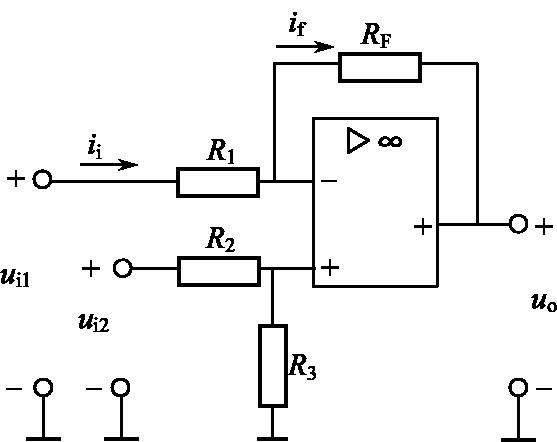
\includegraphics[width=0.25\textwidth]{差分减法运算电路.jpg}
    \caption{减法运算电路}
    \label{fig:减法运算电路}
\end{wrapfigure}
\Par 同样我们给出结论
\begin{equation}
    u_o=\left( 1+\frac{R_F}{R_1} \right) \frac{R_3}{R_2+R_3}u_{12}-\frac{R_F}{R_1}u_{11}
\end{equation}
当$R_1=R_2,R_F=R_3$,我们就实现了减法的功能
\begin{equation}
    u_o=\left( 1+\frac{R_F}{R_1} \right) \frac{R_F}{R_1+R_F}u_{12}-\frac{R_F}{R_1}u_{11}=\frac{R_F}{R_1}\left( u_{12}-u_{11} \right) 
\end{equation}
当然,如果令$R_1=R_2=R_F=R_3$,那么就有
\begin{equation}
    u_o=u_{12}-u_{11}
\end{equation}